\documentclass[11pt,a4paper]{article}

\usepackage[margin=0.2in]{geometry}
\usepackage[utf8]{inputenc}
\usepackage[MeX]{polski}
\usepackage{graphicx}
\usepackage{wrapfig}
\usepackage{color}
\usepackage{amsmath}
\usepackage{amssymb}
\usepackage[inkscapelatex=false]{svg}
\usepackage{array, makecell}
\usepackage{mhchem}
\usepackage{tabularx}
\usepackage{braket}
\usepackage{pdfpages}

\usepackage{multicol}
\usepackage{colortbl}
\usepackage[Export]{adjustbox}
\adjustboxset{max size={0.9\linewidth}{0.9\paperheight}}
\usepackage[colorlinks=true,linkcolor=red,citecolor=green]{hyperref}

\textwidth=16cm
\textheight=23cm
\topmargin=-2cm
\oddsidemargin=0cm

\setlength{\parindent}{0em}
\setlength{\parskip}{0.6em}
\setlength{\jot}{12pt}

\renewcommand{\arraystretch}{1.4}
\renewcommand\theadfont{\bfseries}

\newcommand{\todo}[1]{\textcolor{red}{TODO: #1}}

\begin{document}

\title{\textbf{KMS\\Symulacja dynamiki kwantowej cząstki}}
\author{Dawid Karpiński}
\date{20.12.2023 r.}
\maketitle
\pagebreak

\section{Test symulacji}

\begin{figure}[ht!]
    \caption{\textbf{Średnia energia od czasu dla niestabilnych kroków $d\tau$}}
    \vspace{0.2cm}
    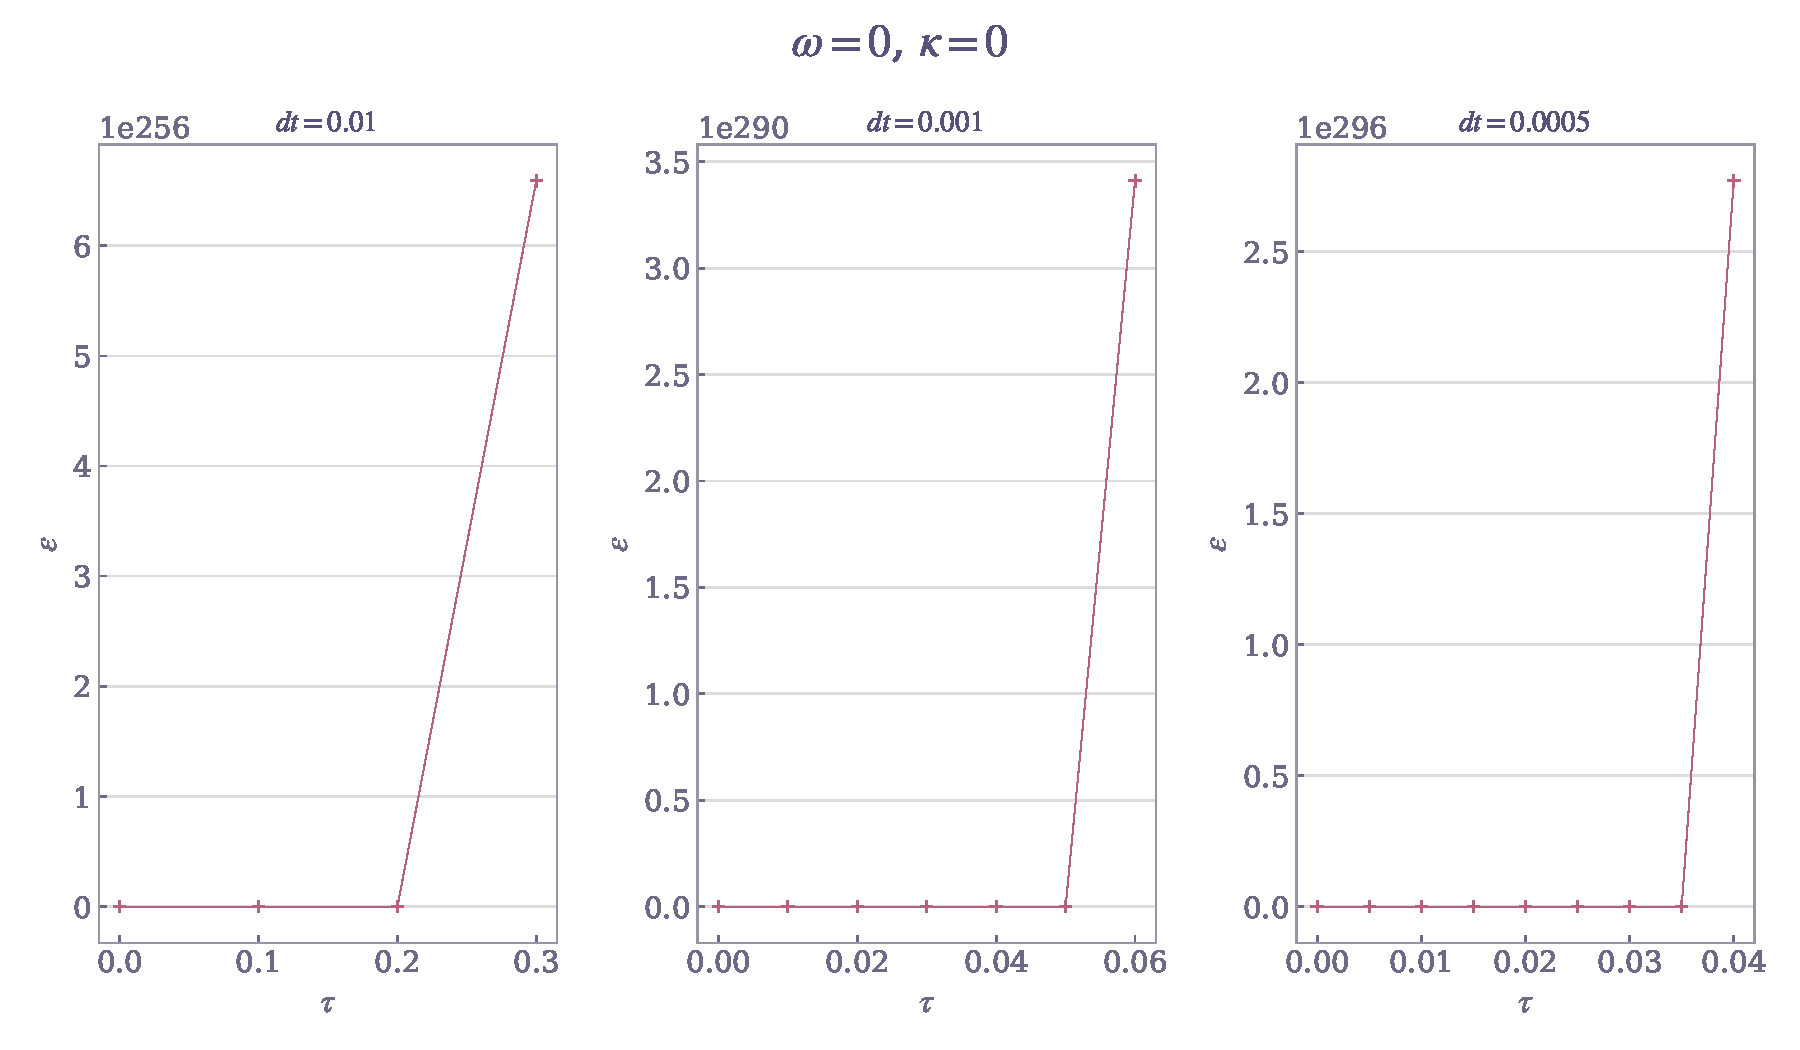
\includegraphics[width=\linewidth]{../figures/unstable.pdf}
\end{figure}

Symulacja okazała się być stabilna tylko dla kroku $d\tau=0.0001$. Inne zbadane kroki powodowały, że symulacja była mocno niestabilna (średnia energia dążyła szybko do nieskończoności).

\begin{figure}[ht!]
    \caption{\textbf{Zależności od czasu dla: normy $\mathcal{N}$, średniego położenia $x$, średniej energii $\varepsilon$ (brak zaburzenia)}}
    \vspace{0.2cm}
    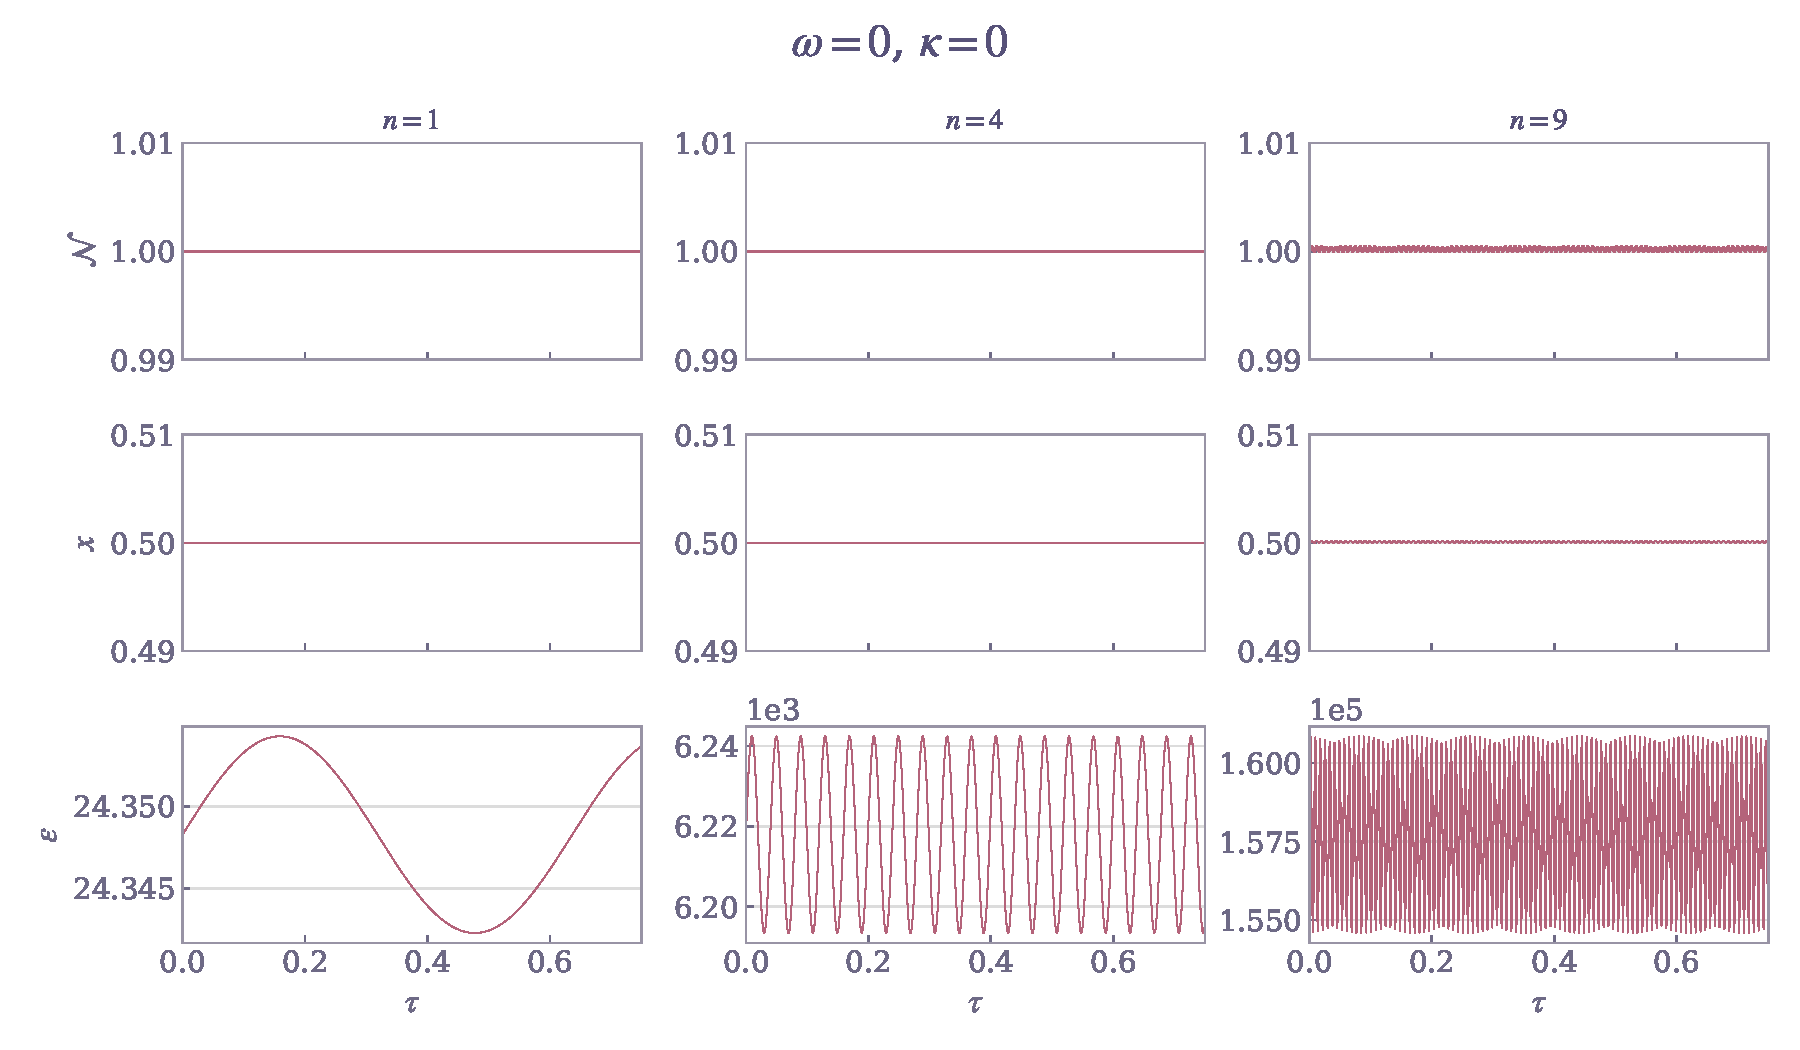
\includegraphics[width=\linewidth]{../figures/stationary.pdf}
\end{figure}

\begin{figure}[ht!]
    \caption{\textbf{Zależności od czasu dla: normy $\mathcal{N}$, średniego położenia $x$, średniej energii $\varepsilon$ (z zaburzeniem)}}
    \vspace{0.2cm}
    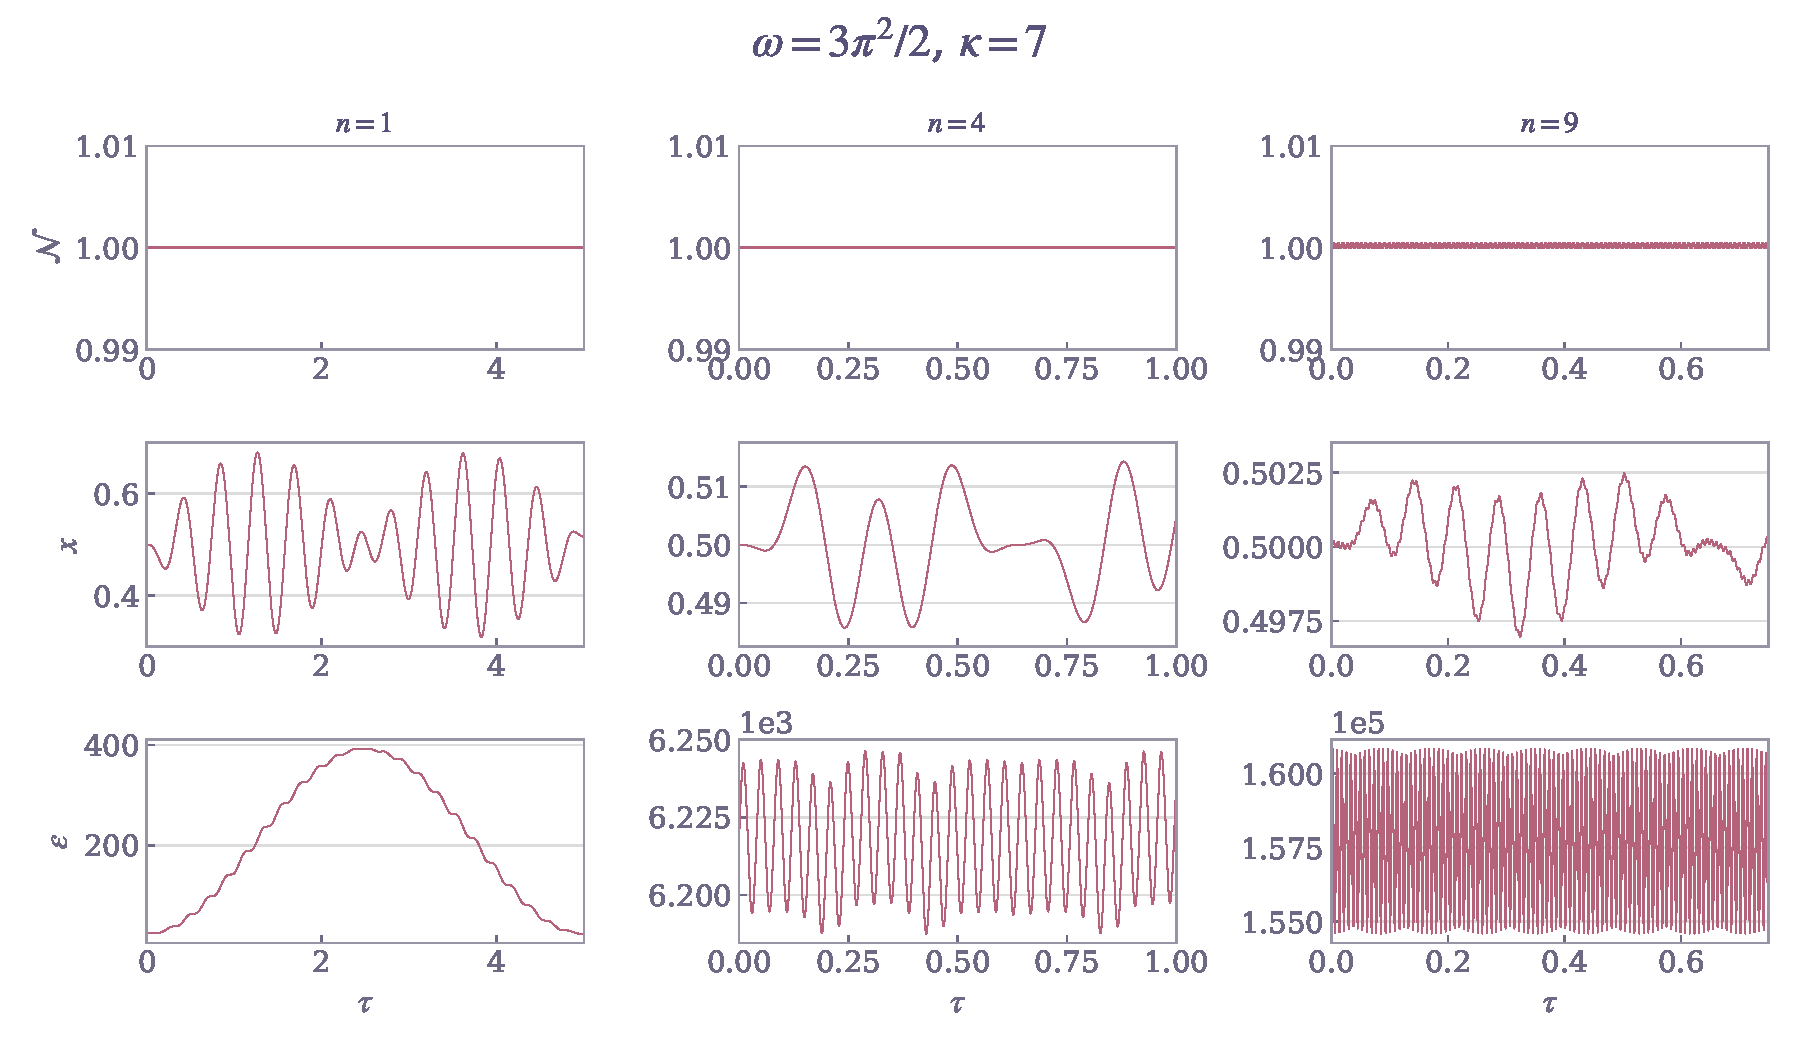
\includegraphics[width=\linewidth]{../figures/fluctuations.pdf}
\end{figure}
\pagebreak

\section{Badanie rezonansu}

\begin{figure}[ht!]
    \caption{\textbf{Skan wartości $\omega$ w poszukiwaniu rezonansu}}
    \vspace{0.2cm}
    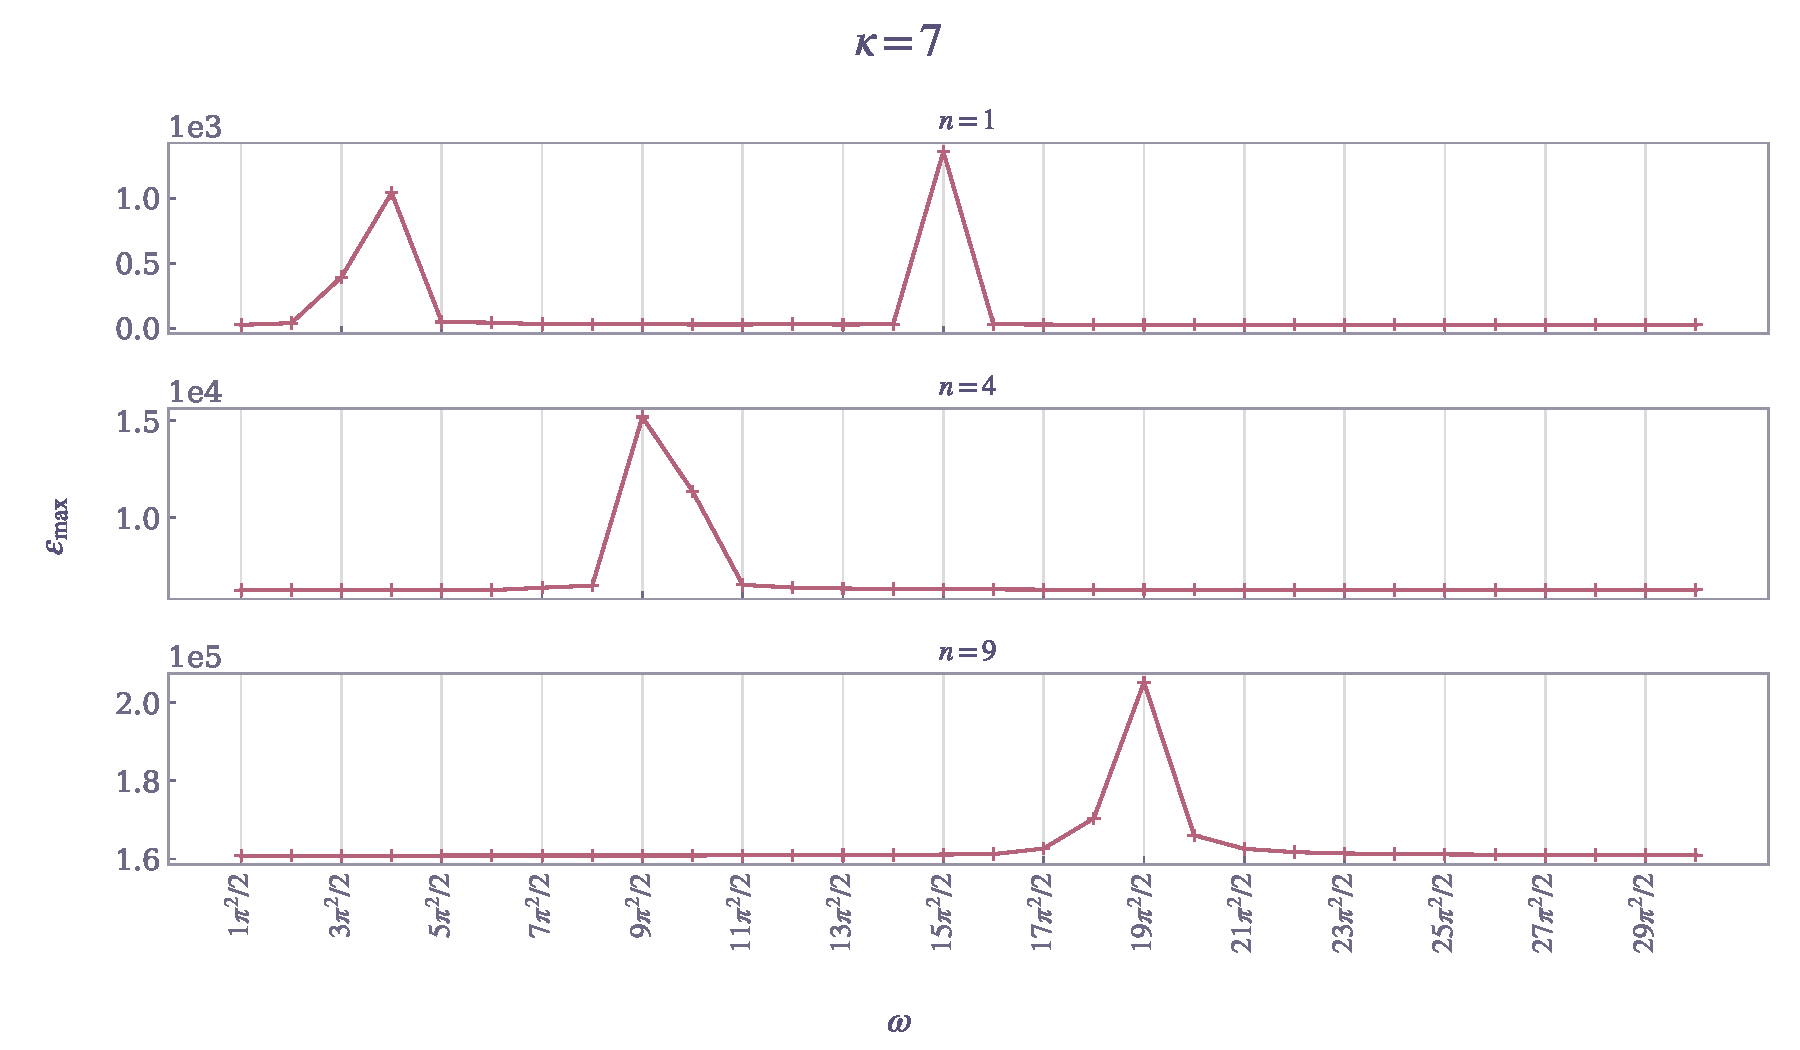
\includegraphics[width=\linewidth]{../figures/resonance.pdf}
\end{figure}

Wartości $\omega$ dla których zachodzi rezonans znaleziono poprzez wykonanie skanu 30 punktów pomiarowych. Zbadano miejsca w których zaobserwowano pik.
\pagebreak

\begin{table}[h!]
\vspace{1.5cm}
\begin{center}
\begin{tabular}{|| c | c | c | c ||}
    \hline
    $\omega$ & stan własny / przejście & rezonans & t\\
    \hline
    $\frac{1\pi^2}{2}$ & 1 & nie & -\\
    \hline
    $\frac{2\pi^2}{2}$ & 1 & nie & -\\
    \hline
    $\frac{3\pi^2}{2}$ & 1 / $1\rightarrow2$ & tak & 1.5\\
    \hline
    $\frac{4\pi^2}{2}$ & 1 & nie & -\\
    \hline
    $\frac{5\pi^2}{2}$ & 1 & nie & -\\
    \hline
    \hline
    $\frac{14\pi^2}{2}$ & 1 & nie & -\\
    \hline
    $\frac{15\pi^2}{2}$ & $1\rightarrow2$ & tak & 4.0\\
    \hline
    $\frac{16\pi^2}{2}$ & 1 & nie & -\\
    \hline
\end{tabular}
\caption{$n=1$}
\end{center}
\end{table}

\begin{figure}[ht!]
    \centering
    \begin{multicols}{3}
        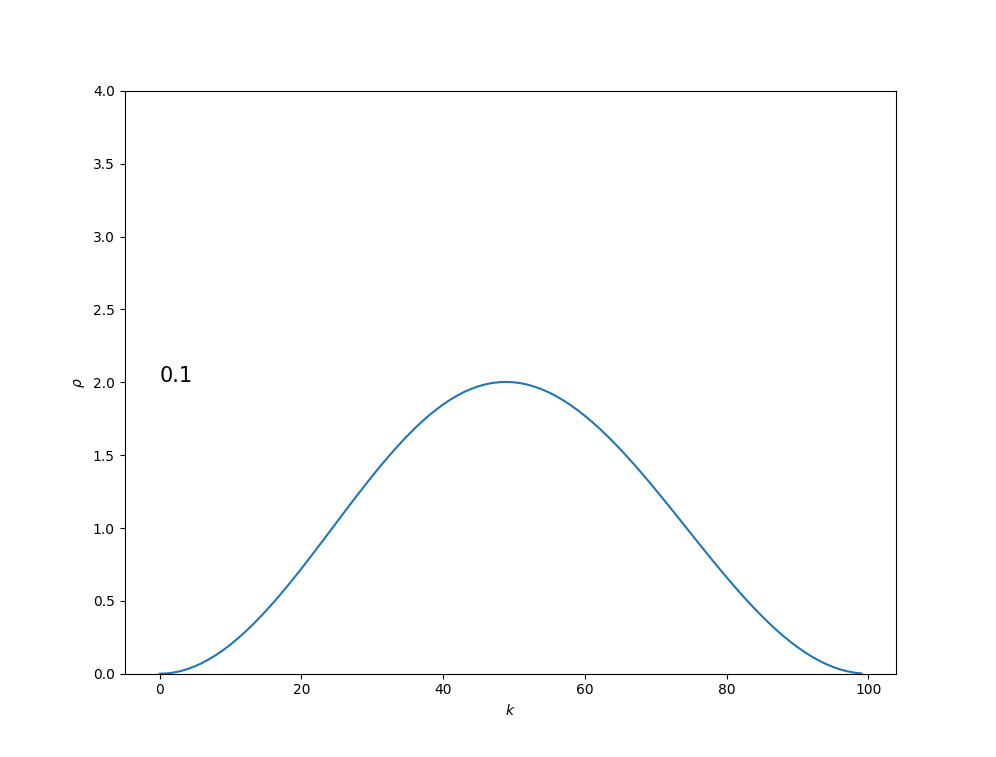
\includegraphics[width=\linewidth]{../figures/frame_n=1_time=0.1.png}
        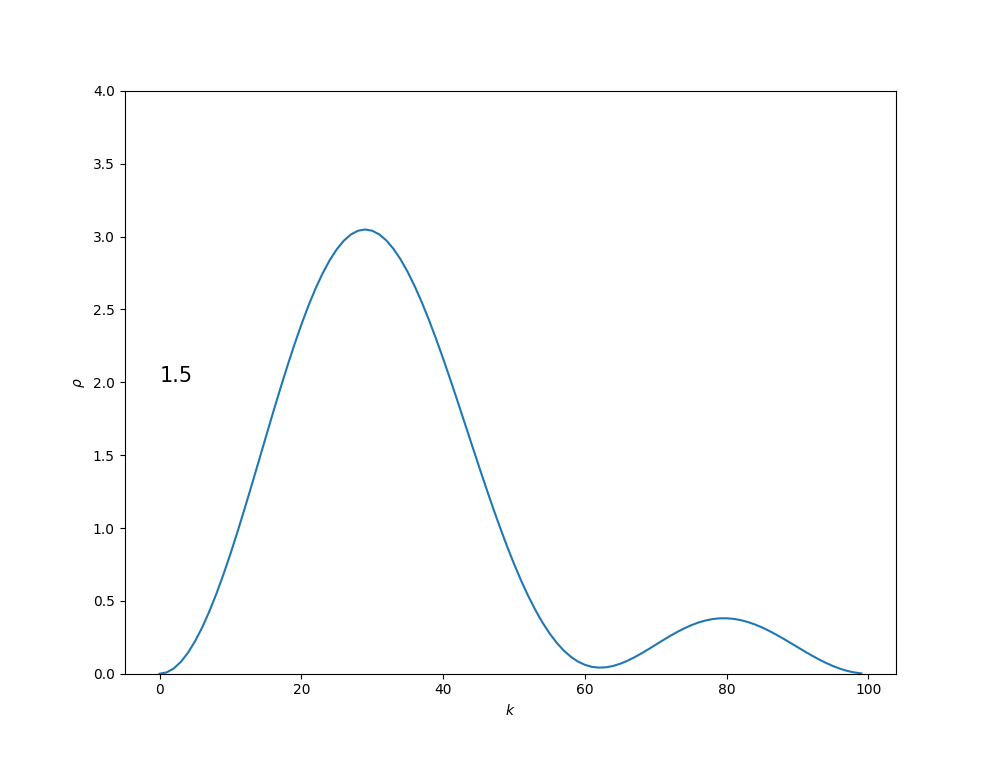
\includegraphics[width=\linewidth]{../figures/frame_n=1_time=1.5.png}
        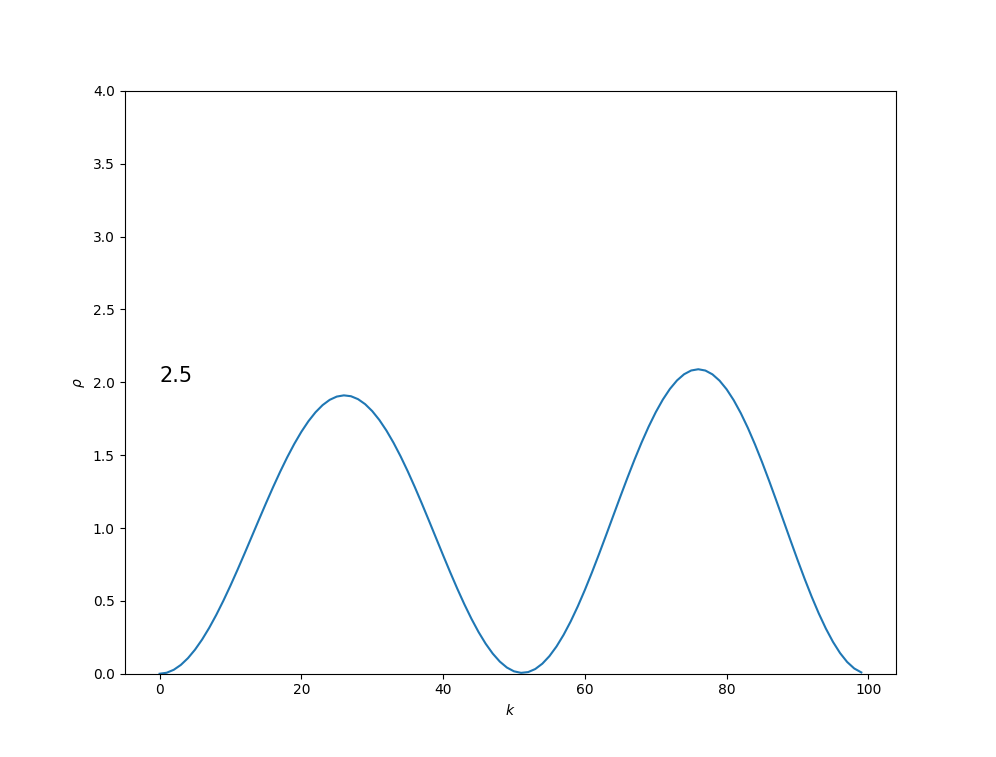
\includegraphics[width=\linewidth]{../figures/frame_n=1_time=2.5.png}
    \end{multicols}
    \caption{\textbf{Zachowanie gęstości w różnych krokach czasowych dla $n=1$, od lewej: $t=0.1,1.5,2.5$}}
\end{figure}
\pagebreak

\begin{table}[h!]
\vspace{1.5cm}
\begin{center}
\begin{tabular}{|| c | c | c | c ||}
    \hline
    $\omega$ & stan własny / przejście & rezonans & t\\
    \hline
    $\frac{7\pi^2}{2}$ & 4 & nie & -\\
    \hline
    $\frac{8\pi^2}{2}$ & 4 & nie & -\\
    \hline
    $\frac{9\pi^2}{2}$ & 4 / $4\rightarrow5$ & tak & 2.0\\
    \hline
    $\frac{10\pi^2}{2}$ & 4 & nie & -\\
    \hline
    $\frac{11\pi^2}{2}$ & 4 & nie & -\\
    \hline
\end{tabular}
\caption{$n=4$}
\end{center}
\end{table}

\begin{figure}[ht!]
    \centering
    \begin{multicols}{3}
        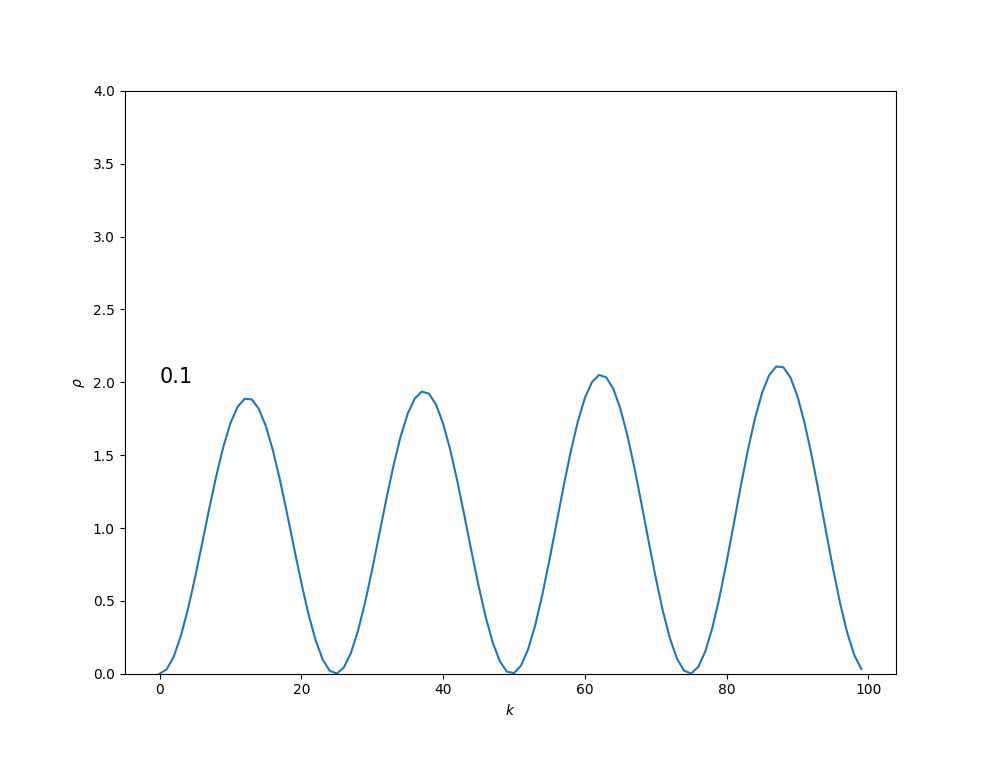
\includegraphics[width=\linewidth]{../figures/frame_n=4_time=0.1.png}
        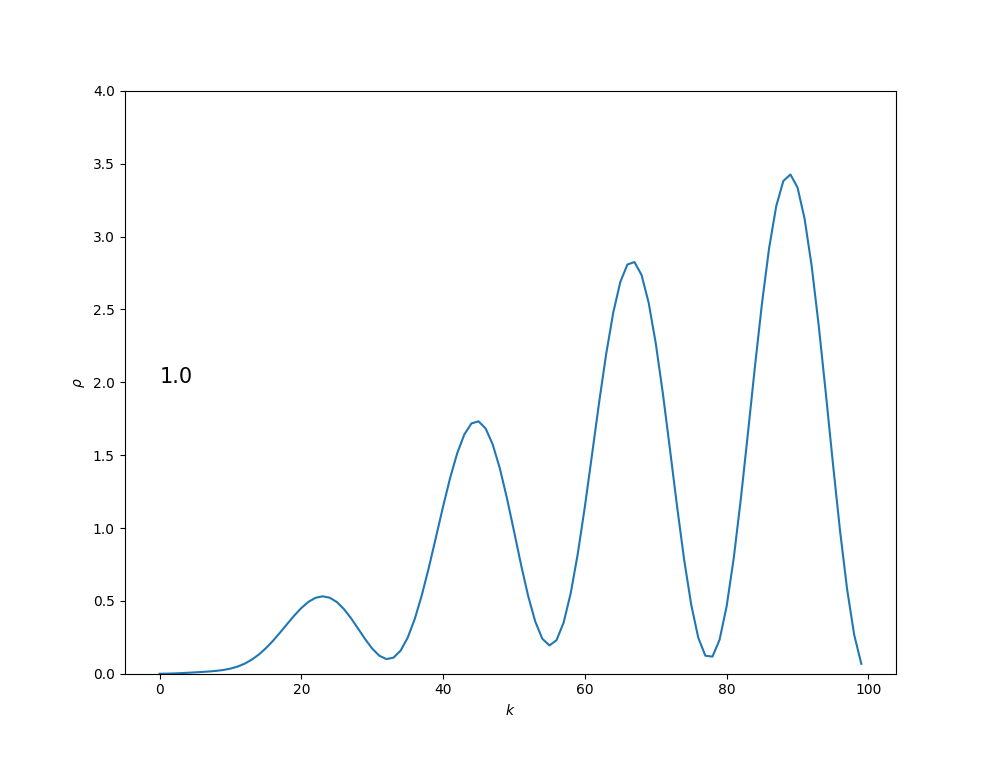
\includegraphics[width=\linewidth]{../figures/frame_n=4_time=1.0.png}
        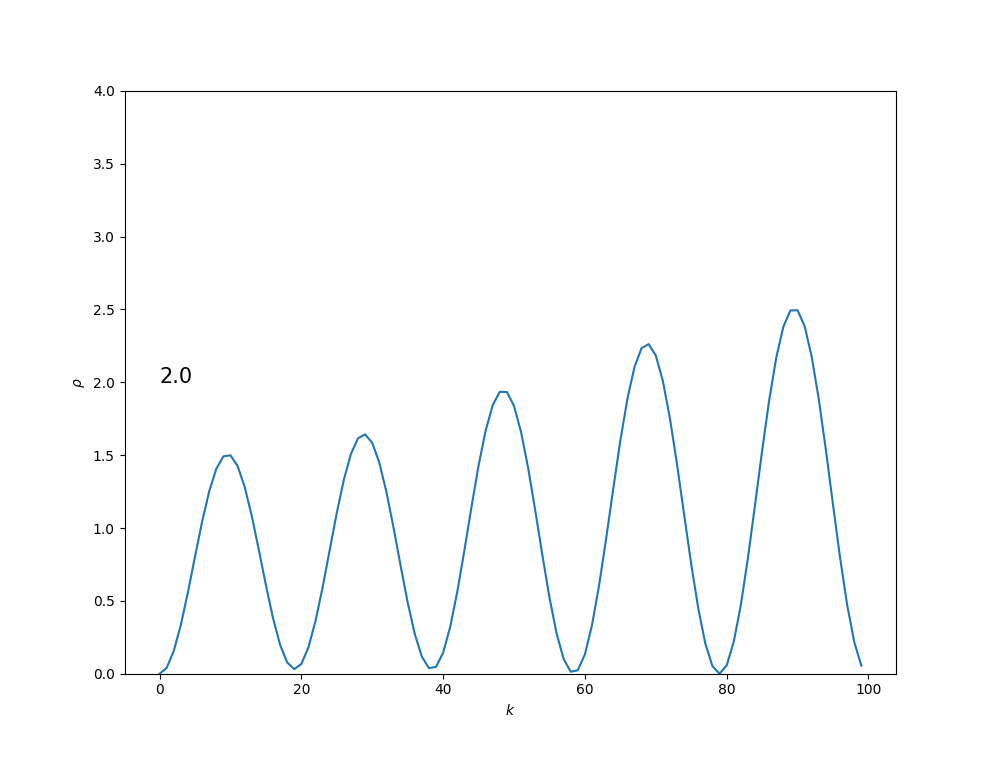
\includegraphics[width=\linewidth]{../figures/frame_n=4_time=2.0.png}
    \end{multicols}
    \caption{\textbf{Zachowanie gęstości w różnych krokach czasowych dla $n=4$, od lewej: $t=0.1,1.0,2.0$}}
\end{figure}
\pagebreak


\begin{table}[h!]
\vspace{1.5cm}
\begin{center}
\begin{tabular}{|| c | c | c | c ||}
    \hline
    $\omega$ & stan własny / przejście & rezonans & t\\
    \hline
    $\frac{17\pi^2}{2}$ & 9 & nie & -\\
    \hline
    $\frac{18\pi^2}{2}$ & 9 & nie & -\\
    \hline
    $\frac{19\pi^2}{2}$ & 9 / $9\rightarrow10$ & tak & 2.0\\
    \hline
    $\frac{20\pi^2}{2}$ & 9 & nie & -\\
    \hline
    $\frac{21\pi^2}{2}$ & 9 & nie & -\\
    \hline
\end{tabular}
\caption{$n=9$}
\end{center}
\end{table}

\begin{figure}[ht!]
    \centering
    \begin{multicols}{3}
        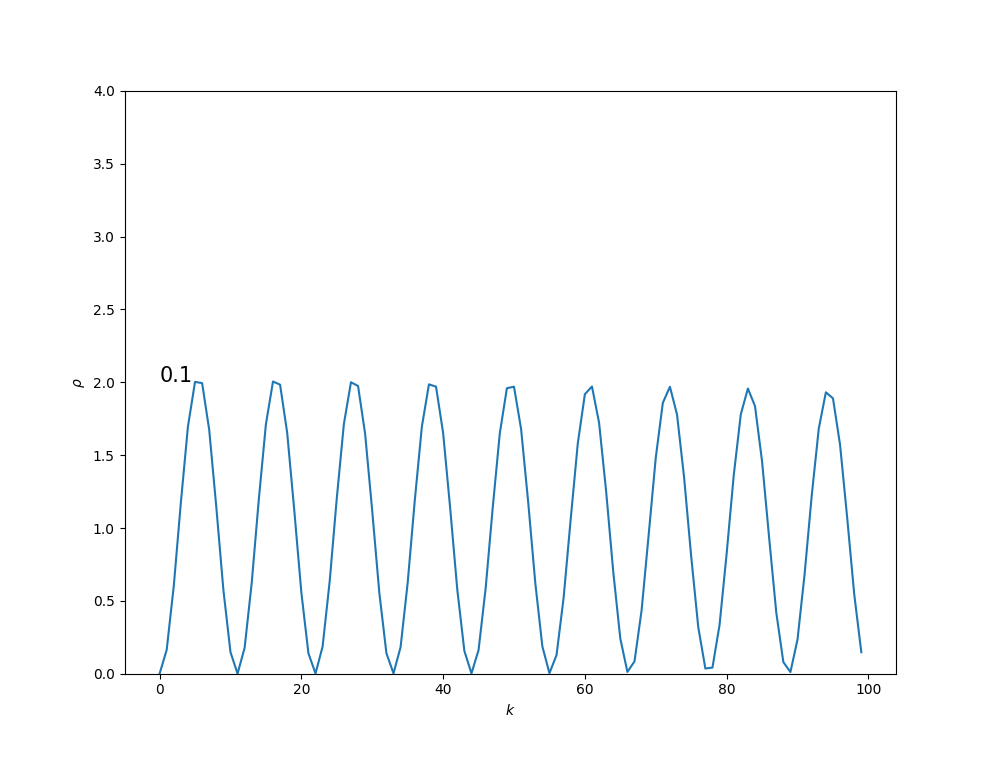
\includegraphics[width=\linewidth]{../figures/frame_n=9_time=0.1.png}
        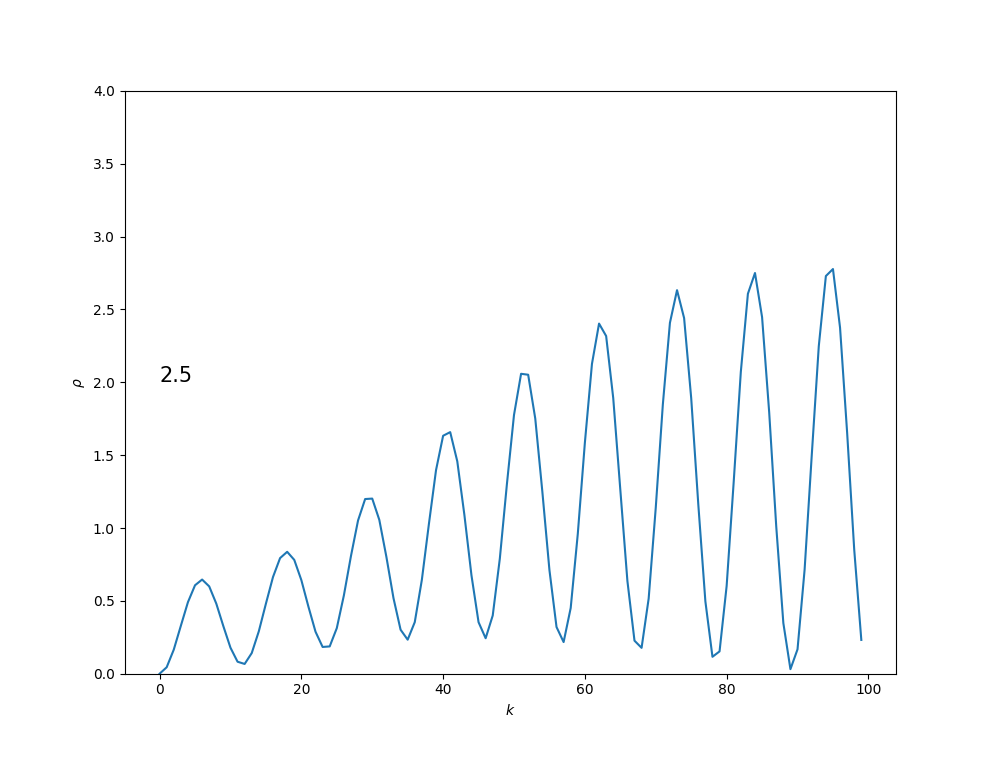
\includegraphics[width=\linewidth]{../figures/frame_n=9_time=2.5.png}
        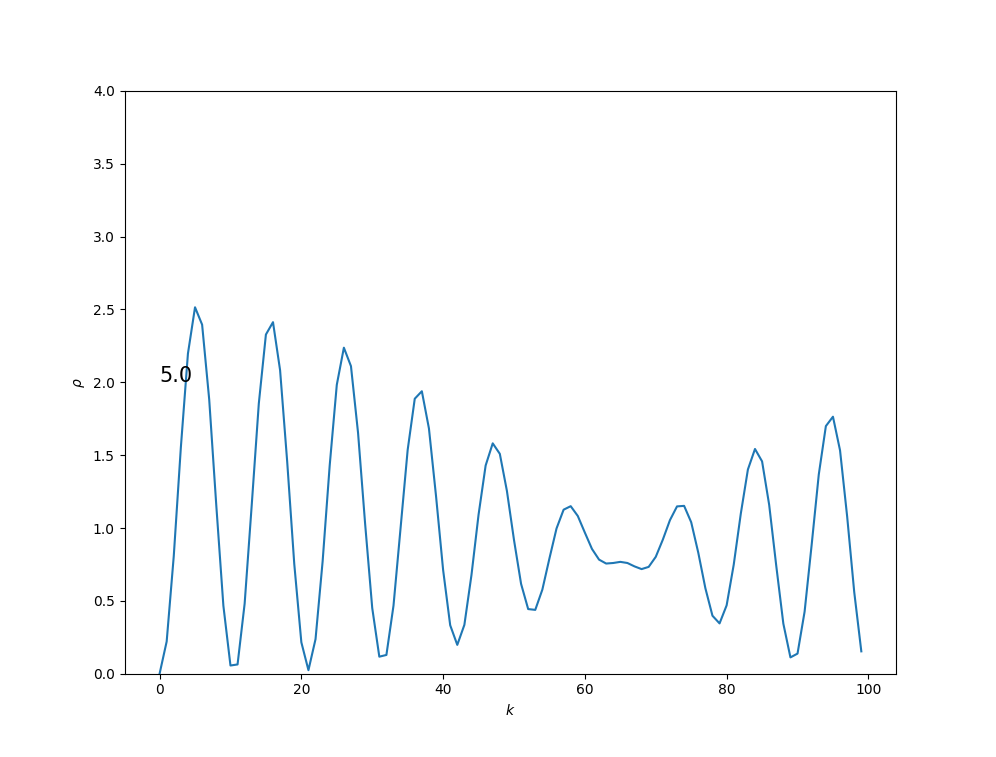
\includegraphics[width=\linewidth]{../figures/frame_n=9_time=5.0.png}
    \end{multicols}
    \caption{\textbf{Zachowanie gęstości w różnych krokach czasowych dla $n=9$, od lewej: $t=0.1,2.5,5.0$}}
\end{figure}
\clearpage

\section{Wnioski}

W pierwszym etapie symulacji sprawdzono poprawność algorytmu. Wykonano obliczenia dla stanów cząstkowych o numerach 1, 4 i 9, monitorując normę, średnie położenie i średnią energię.

W dalszych symulacjach wprowadzono zaburzające pole zewnętrzne. Przeprowadzono symulacje dla różnych wartości częstotliwości rezonansowej $\omega$. Czas symulacji ustawiono tak, aby obejmował co najmniej jeden pełny cykl okresowych zmian energii.

Do wykonania symulacji zastosowano język F\#, a do wizualizacji Python/Matplotlib.

\end{document}
